\documentclass[a4paper, 11pt]{jsreport}%サイズ変更12->11
\usepackage{bm}
\usepackage[dvipdfmx]{graphicx}
\usepackage{ascmac}
\usepackage{wrapfig}
\usepackage{here}
\usepackage{url}
\usepackage[normalem]{ulem}
\usepackage[dvipdfmx, bookmarkstype=toc, colorlinks=false, pdfborder={0 0 0}, bookmarks=true, bookmarksnumbered=true]{hyperref}
\usepackage{pxjahyper}
\usepackage{caption}%追加部分
\captionsetup{font={footnotesize,bf}, labelsep=space}%追加部分

\makeatletter

%日本語
\def\@thesis{卒業論文}
\def\id#1{\def\@id{#1}}
\def\department#1{\def\@department{#1}}
\def\prof#1{\def\@prof{#1}}

%English
\def\departmenten#1{\def\@departmenten{#1}}
\def\profen#1{\def\@profen{#1}}
\def\titleen#1{\def\@titleen{#1}}
\def\authoren#1{\def\@authoren{#1}}
\def\dateen#1{\def\@dateen{#1}}

%要編集
\title{
    VR空間における音源の空間的配置が\\音程識別学習に与える影響
}

\titleen{
    The Effect of Spatial Sound Source Placement on Pitch Interval Identification in VR Environments
}
\department{
    % 所属学科
    早稲田大学基幹理工学部\\
    情報理工学科
}
\author{
    % 自分の名前(日本語)
    内藤　光志
}
\authoren{
    % 自分の名前(英語)
    Koji Naito
}
\id{
    % 学籍番号
    1W222257-8
}
\prof{
    % 教授の名前(日本語)
    中島　達夫
}
\profen{
    % 教授の名前(英語)
    Professor Tatsuo Nakajima
}
\dateen{
    % 発行日
    \today
}

%日本語タイトル(編集不要)
\newcommand{\maketitlejp}{
    \begin{figure}[t]
        \centering
        
\includegraphics[keepaspectratio, scale=0.6]{kousyou.png}
    \end{figure}
    \begin{center}
        {\huge \@thesis \par}
        \vspace{20mm}
        {\huge \@title \par}
        \vspace{13mm}
        {\LARGE \@department \par}
        \vspace{10mm}
        {\huge \@author \par}
        \vspace{10mm}
        {\LARGE \hspace{28mm}学籍番号\hfill\@id\hspace{28mm} \par}
        {\LARGE \hspace{28mm}提出\hfill\@date\hspace{28mm} \par}
        {\LARGE \hspace{28mm}指導教授\hfill\@prof\hspace{28mm} \par}
    \end{center}
    \par\vskip 1.5em
}

%英語タイトル(編集不要)
\newcommand{\maketitleen}{
    \clearpage %追加
    \begin{center}
        \vspace{10mm}
        {\Huge \bf \@titleen \par}
        \vspace{20mm}
        {\LARGE \@authoren \par}
        \vspace{20mm}
        {\Large Thesis submitted in partial fulfillment of\\the requirements for the degree of \par}
        {\LARGE Bachelor in Computer Science \par}
        \vspace{15mm}
        {\LARGE \uline{\hspace{7mm}Student ID\hfill\@id\hspace{7mm}} \par}
        {\LARGE \uline{\hspace{7mm}Submission Date\hfill\@dateen\hspace{7mm}} \par}
        {\LARGE \uline{\hspace{7mm}Supervisor\hfill\@profen\hspace{7mm}} \par}
        \vspace{10mm}
    \end{center}

    \begin{wrapfigure}[4]{r}{15mm}
        
\includegraphics[width=2.3cm]{kousyou.png}
    \end{wrapfigure}

    \large \hfill \par \hfill Department of Computer Science and Engineering\\\hfill School of Fundamental Science and Engineering\\\hfill Waseda University
}

\makeatother
\setcounter{tocdepth}{3} %追加



\begin{document}
\maketitlejp
\maketitleen

\newpage
\addcontentsline{toc}{chapter}{概要}
\begin{center}
\Large{概要}
\end{center}

聴音トレーニングとは，聴覚を用いて音程やリズム等の音楽的要素を識別するトレーニングで，こうしたトレーニングによる音程認識能力の習得は音楽教育の基盤である．これまで，本訓練は指導者に依存していたが，近年ではソフトウェアによる独習へと移行してきており，Virtual Reality（VR）技術を用いた多感覚的アプローチが注目されている．特に，VR特有の空間音響は音程認識の新たな手がかりとなり，従来の学習環境よりも高い学習効果をもたらす可能性が示唆されている．さらに、既存の平面的なディスプレイを用いた学習では，視覚と聴覚の連携は限定的であり，実空間での音源定位や身体性を伴う知覚体験は提供されていない。そこで本研究では、人間が持つ音高の変化を空間的な「高さ」や「配置」として認知する特性を活用し、VR 空間において音源を立体的に配置することで，この空間認知能力を聴音学習に直接的に利用するアプローチに注目した。これにより、単なる知識の習得を超え，音程を直感的かつ身体的に捉える新たな認知スキームの獲得につながると考えられる．


そこで，本研究では，VR空間内で音源を立体的に配置することで学習者に与える影響を明らかにすることを目的とし，VR技術を適用した聴音トレーニングの音源配置の違いについて検討を行った．具体的には，既存手法である平面的インターフェースに対応した前方半円状に音源を配置するシステムと，新たに提案する音の高さを空間的距離や方位に拡張させた円状配置システムといった2つのシステム間で，NASA-TLXによる作業負荷やテスト時間，正答率を比較検証した．


\newpage
\addcontentsline{toc}{chapter}{Abstract}
\input{Text/0-AbstractEn}


\tableofcontents %目次
\listoffigures %図目次
\listoftables %表目次

%%%第1章%%%
\chapter{序論}
\section{背景} \label{sec:background}
聴音トレーニング（Ear Training）とは，聴覚を用いて音高，音程，旋律，和音，リズムといった音楽的要素を識別する技術を習得するための訓練である．これは音楽家の育成において極めて重要な役割を果たしており，その最終的な到達点は，聴覚のみを用いて音楽を正確に表現し，伝達する「インナーヒアリング」の獲得にある\cite{woody2012playing}．この文献で，多様な形態が提案されているが，こうした聴覚能力の獲得における基礎は旋律の認識であり，そのためには構成音間の「音程」を区別し認識する能力を重要視している．したがって，音程認識能力の向上は，音楽学習者が優れたインナーヒアリングを獲得するための最も基礎的な手段であるといえる．

従来，聴音トレーニングは指導者やパートナーがピアノ等で課題を演奏し，学習者の回答を評価するという人的リソースに依存した形式で行われてきた．しかし，計算機技術の発展に伴い，様々な訓練用ソフトウェアが開発されている．その歴史は古く，1970年代半ばにはPLATOメインフレーム上で動作する「G.U.I.D.O.」\footnote{https://www.learntechlib.org/p/168759/}が開発され，大学の音楽学生向けに音程・旋律・和音等の認識指導が行われた．また，1996年にリリースされた「EarMaster」\footnote{https://www.earmaster.jp/}は，現在でも広く利用されている代表的なソフトウェアであり，音程比較からリズム認識まで多岐にわたるトレーニング機能を提供している．これらはスタンドアロン，Webブラウザ，モバイルデバイスなど多様なプラットフォームで利用可能であり，独習の機会を広げている．

さらに，近年急速に普及しているVirtual Reality（VR）技術は，視覚，聴覚，触覚を含む多感覚入力を統合した仮想環境（Virtual Environments）を提供する技術である．SerafinらによりこうしたVRおよびAR（拡張現実）の技術とソフトウェアについて音楽教育分野に関する包括的なレビューが行われている\cite{serafin2017considerations}．また現在VRでの音楽教育分野における研究として特定の楽器における楽器支援\cite{gao2024application}や、既存の音楽レッスンによる拡張\cite{liu2025research}が挙げられ，本研究は後者に位置づけられる．こうした研究がVRを扱う利点として高価な機器の準備や教師不足が挙げられている．またVRは既存のウェブアプリケーションよりも空間的要素を高めることができ，音楽学習者が楽器の演奏や視聴における近しい体験が提供できる利点もある．また現在の聴音トレーニングにおけるインターフェースの多くはピアノの鍵盤のような「水平・平面的な配置」に依存している．PedersonらはVRでの聴音トレーニングにおいて、ステレオ音響を音程認識の手がかりとして影響を与えていることが示唆されている\cite{pedersen2020spatialized}。これはステレオ音響がVR技術での学習において有益である可能性について期待できる．従来の平面的なインターフェースに対し，音のピッチ（高低）は空間的な高低に対して結びついていることが示されており\cite{rusconi2006spatial}，VR空間であれば，物理的な制約を受けずに，この「音の高さ」と「空間的な高さ」を一致させた立体的な音源配置が可能である．

そこで本研究では，VR技術を用いた聴音トレーニングについて，既存手法\cite{pedersen2020spatialized, fletcher2019virtual}である平面的インターフェースを模した前方半円状配置と，音程の周波数を空間の距離に対応させた円状配置したシステムにおける聴音トレーニングを比較検討することで，音楽教育分野のさらなる発展に向けた可能性を模索する．

\section{研究目的}
本研究の目的は，VR空間内の聴音トレーニングにおいて，音源を立体的に配置することが学習者の音程認識に与える影響を明らかにすることである．平面的なインターフェースとして前方半円状配置と，音程の周波数に基づく音源の高さの調整を行った円状配置の2つのシステムを用いた．18名を実験参加者とし，それぞれの音楽経験を考慮した上での，2つの音が順になり「ピッチインターバル（音程識別」を聞き分けるテストを行い，さらなる評価を行っている．本研究の成果は，将来的なVR音楽教育システムの設計において，更なる発展に寄与することを目指す．

\section{論文構成}
本論文の構成は以下の通りである．\\

第1章　序論

　本研究の背景および研究目的について述べる．

第2章　関連研究

　本研究に関連する研究について述べる．\\

第3章　設計

　実験に使用したゲームの設計について述べる．

第4章　実験

　実施した評価実験について述べる．

第5章　結果

　評価実験にて得られた結果について示す．

第6章　考察

　結果に基づいた考察を述べる．

第7章　結論

　本研究の結論と将来課題について述べる．

%%%第２章%%%
\chapter{関連研究}
\input{Text/2-RelatedWork}


%%%第3章%%%
\chapter{設計}
\section{システムの概要}
本システムは，VR環境を活用し，仮想音源の音高（ピッチ）と空間的な位置関係を結びつけることで，聴覚と空間認識能力の向上を目指すVR学習支援アプリケーションである．学習の基盤として，12個の仮想音源（球体）を，視覚情報が集中する前方半円状に配置する「180度配置」と，全方位に配置する「360度配置」の2パターンを設定可能とし，学習目的に応じた柔軟なトレーニングを提供する．音源には，ピッチ識別が容易なピアノ音を採用しており\cite{pedersen2020spatialized}，これによりユーザは空間的な位置と特定のピッチとの対応関係を正確かつ効率的に習得することが期待される．
\section{使用機材}
本システムはヘッドマウントディスプレイ（HMD）により視覚，聴覚刺激を提示し，コントローラによる触覚刺激を利用する．HMDにはMeta Quest 2，コントローラにはMeta Quest 2のコントローラを用いた．また，アプリケーションの開発環境にはUnity 6を使用した．使用したHMDおよびコントローラを図\ref{fig:hardware}に示す．

\begin{figure}[H]\centering
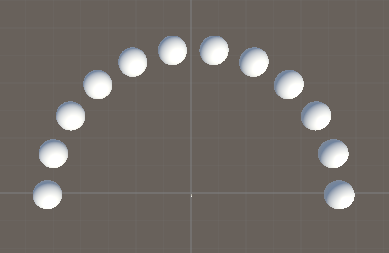
\includegraphics[width=100mm]{figure/system_hardware.png}\caption{実験で使用したHMDとコントローラ}\label{fig:system_hardware}
\end{figure}

\section{システムの設計実装}
\subsection{前方円状配置システム}\label{sec:system_180}
本研究で開発した「前方円状配置」システムの概要図を図\ref{fig:system_180_overview}に示す．

\begin{figure}[H]\centering
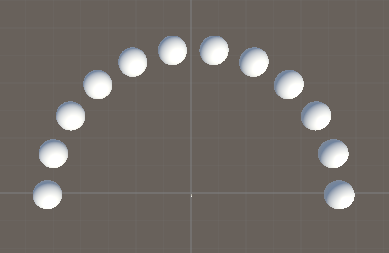
\includegraphics[width=100mm]{figure/system_180.png}\caption{180度配置}\label{fig:system_180_overview}
\end{figure}

180度配置の空間は，既存の音感トレーニングシステムを模した条件である．ユーザの前方を中心とした半円周上（水平角 $-90$度 $\sim$ $+90$度）に，12個の音源を等間隔に配置した．隣接する音源同士の角度間隔は約15度であり，音源密度が高い状態となっている．なお，音源の高さ（Y軸座標）については，一般的な鍵盤配置を想定し，全ての音源をユーザの耳の高さ（$Y=0$）で一定とした．

\subsection{全方位配置システム}\label{sec:system_360}
次に，本研究で提案する「全方位配置」システムの概要図を図\ref{fig:system_360_overview}および図\ref{fig:system_360_height}に示す．

\begin{figure}[H]\centering
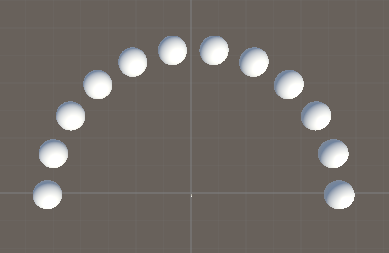
\includegraphics[width=100mm]{figure/system_360.png}\caption{上から見た360度配置}\label{fig:system_360_overview}
\end{figure}

\begin{figure}[H]\centering
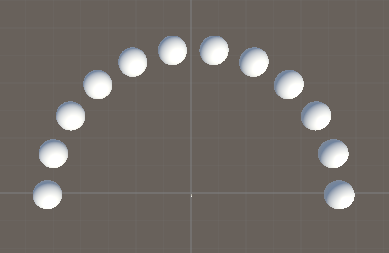
\includegraphics[width=100mm]{figure/system_360.png}\caption{横から見た360度配置}\label{fig:system_360_height}
\end{figure}

図3.3で示した全方位配置は，本研究で提案する全周囲を活用した条件である．基準音（C3）から1オクターブ上の音（B3）までの全12音（半音階）を配置対象とし，各音源オブジェクトはユーザを中心として等距離・等間隔に配置される．音源の高さ（Y軸座標）については，音高の上昇に伴って螺旋状に上昇する配置を採用した．この際，音源間の距離設定には音階ごとの周波数比を用い，以下の式を適用した．

\begin{equation}
    d = d_0 \times \frac{f}{f_0}\label{eq:dist_linear}
\end{equation}

ここで，$d$は中心から対象音源までの距離，$d_0$は中心から基準音までの距離，$f$は対象音源の周波数，$f_0$は基準音の周波数である．また，周波数は以下の式で平均律に基づく音名に割り当てることができる．

\begin{equation}
    f = f_0 \times (2)^{\frac{n}{12}} \label{eq:freq_linear}
\end{equation}

ここで，$n$は基準音からの半音数，$f$は基準音から$n$半音上の音の周波数，$f_0$は基準音の周波数である．この式に従い，周波数の物理的な変化（Hzの増加）をそのまま空間的な距離の比率として変換を行っている．

\subsection{システムの共通機能}
\ref{sec:system_180}および\ref{sec:system_360}で述べた2つのシステムに共通する機能について説明する．本システムにはPractice ModeとTest Modeの2つのモードが存在する．Training Modeでは，ユーザが任意の音源オブジェクトをコントローラで選択することで，対応する音高の音が再生される．これにより，ユーザは各音源の位置と音高の対応関係を自由に確認できる．一方，Test Modeでは，ピッチインターバルをTraining Modeで確認している音源の配置にしたがい，ユーザはその位置に対応する音源オブジェクトをコントローラで選択することで回答を行う．問題数は全部で24問あり，正解・不正解のフィードバックは選択した瞬間にUIとして表示されるように設計した，ユーザは自身の回答結果を後で確認できる．また，Test Modeでは各モード終了後に正答率が表示される．さらに，両モードともに，コントローラの振動機能を用いて触覚フィードバックを提供する．ユーザが音源オブジェクトに近づくと振動強度が増加し，遠ざかると減少する仕組みとなっている．


\chapter{実験}

本章では、本研究にて実施した実験の方法について述べる。

\section{実験参加者}
実験参加者は合計18名（男性11名、女性7名）で、年齢は21歳から26歳（平均年齢 22.7歳、標準偏差 1.37）であった。全ての参加者は聴力および視力（矯正視力含む）に異常がないことを自己申告により確認し、実験の目的および手順、安全性のリスク（VR酔い等）について十分な説明を受けた上で、書面による同意を得て実験に参加した。
実験結果に影響を与える可能性のある個人の属性として、音楽経験およびVRデバイスの使用経験について事前アンケートを実施した。音楽経験に関しては、「楽器演奏経験が3年以上ある」と回答した経験者が9名、「半年未満（または経験なし）」と回答した未経験者が9名となり、両群が同数となるよう構成された。また、相対音感トレーニングの専門的な受講経験については、16名が「経験なし」と回答し、過去に受講経験がある者は2名のみであった。 　VRデバイスの使用経験に関しては、「日常的に使用している」または「慣れている」「頻繁ではないが慣れている」と回答した者が計13名（約72%）を占め、「数回使用したことがある」が4名、「初めて」が1名であった。このことから、大半の被験者はVR空間での操作に対して一定の順応性を有していたと考えられる。


\section{実験手順}
本実験の所要時間は被験者1名につき約30分である。実験の開始に先立ち、被験者に対して実験概要の説明を行い、現在の体調や聴覚に関する1〜2分程度の事前アンケートを実施する。その後、被験者はHMDおよびコントローラーを装着し、実験タスクへと移行する。
本実験では、前方範囲のみを使用する180度環境と、周囲全体を使用する360度環境の2つの条件において聴取実験を行う。この際、実験を行う順序によって生じる学習効果や疲労などの順序効果を排除するため、180度環境と360度環境のどちらを先に行うかは被験者ごとにランダムに決定し、カウンターバランスをとる設計とした。また、2つの条件の間には適度な休憩を設け、被験者の状態をリセットした上で次の条件へと進むものとする。
各条件における実験は、まず約5分間の練習を行い、被験者を各環境特有の空間音響や操作方法に十分に習熟させる。続いて、全24回の音階テストを行う。テストフェーズの所要時間は約5分である。両条件の終了後、1〜2分程度の事後アンケートおよびNASA-TLXを用いたシステム負荷の評価を実施し、実験を終了する。

\section{評価手法}
\subsection{定性評価}



\subsection{3つの定量評価}




%%%第4章%%%
\chapter{結果}
\begin{table}[H]\centering
    \caption{フルーツ}
    \begin{tabular}{lrr} \hline
    品名 & 単価(円) & 個数 \\ \hline
    りんご & 100 & 5 \\
    みかん & 50 & 10 \\ \hline
    \end{tabular}
\end{table}


%%%第5章%%%
\chapter{考察}
\input{Text/5-Disccusion}

%%%第6章%%%
\chapter{結論}
\section{結論}


\section{将来課題}



%\addcontentsline{toc}{chapter}{参考文献}
\bibliographystyle{junsrt}
\bibliography{ref} %ref.bibのロード

\newpage
\chapter*{謝辞}
\addcontentsline{toc}{chapter}{謝辞}
\input{Text/9-Acknowledgments}
%謝辞をここに

\newpage
\chapter*{付録}
\addcontentsline{toc}{chapter}{付録}

\end{document}